\section{Auswertung}
\label{sec:Auswertung}

% \begin{figure}
%  \centering
%  \includegraphics{<++>}
%  \caption{<++>}
%  \label{fig:<++>}
% \end{figure}
Für die Auswertung wird Python, im Speziellen Matplotlib \cite{matplotlib}, NumPy \cite{numpy},
SciPy \cite{scipy} und Uncertainties \cite{uncertainties} verwendet.

\subsection{Magnetische Flussdichte einer langen und einer kurzen Spule}
%Tabelle lange Spule
Die verwendete lange Spule hat $\num{300}$ Windungen und eine Länge
von $\SI{24}{\centi\meter}$. %richtige Werte einfügen
Die Werte der magnetischen Flussdichte an den Stellen $x$ inner- und außerhalb
der langen Spule befinden sich in Tabelle \ref{taba1}.
Dieselben Werte sind in Abbildung \ref{plota1} gegeneinander aufgetragen.
\begin{table}\caption{Der magnetische Fluss $B$ an verschiedenen Stellen $x$ in der langen Spule.}
\label{taba1}
\centering
\sisetup{round-mode = places, round-precision=3, round-integer-to-decimal=true}
\begin{tabular}{S[]S[]} 
\toprule
{$B$/ \si{\milli\tesla}} & {$x$/ \si{\centi\meter}}\\
\midrule
0.382 & 0.0\\
0.505 & 0.5\\
0.744 & 1.0\\
0.959 & 1.5\\
1.35 & 2.0\\
1.544 & 2.5\\
1.7619999999999998 & 3.0\\
1.928 & 3.5000000000000004\\
2.024 & 4.0\\
2.093 & 4.5\\
2.1380000000000003 & 5.0\\
2.173 & 5.5\\
2.2030000000000003 & 6.0\\
2.2239999999999998 & 6.5\\
2.238 & 7.000000000000001\\
2.248 & 7.5\\
2.2560000000000002 & 8.0\\
2.262 & 8.5\\
2.265 & 9.0\\
2.2659999999999996 & 9.5\\
2.264 & 10.0\\
2.2560000000000002 & 10.5\\
2.2520000000000002 & 11.0\\
2.247 & 11.5\\
2.241 & 12.0\\
2.231 & 12.5\\
2.219 & 13.0\\
2.221 & 13.5\\
2.222 & 14.000000000000002\\
2.22 & 14.499999999999998\\
2.216 & 15.0\\
2.212 & 15.5\\
2.238 & 16.0\\
2.245 & 16.5\\
2.2230000000000003 & 17.0\\
2.209 & 17.5\\
2.1870000000000003 & 18.0\\
2.1519999999999997 & 18.5\\
2.088 & 19.0\\
2.0 & 19.5\\
1.874 & 20.0\\
1.673 & 20.5\\
1.4469999999999998 & 21.0\\
1.1509999999999998 & 21.5\\
0.82 & 22.0\\
0.575 & 22.5\\
0.416 & 23.0\\
0.303 & 23.5\\
0.221 & 24.0\\
\bottomrule
\end{tabular}\end{table}

%Grafik lange Spule (xB-Diagramm)
\begin{figure}
    \centering
    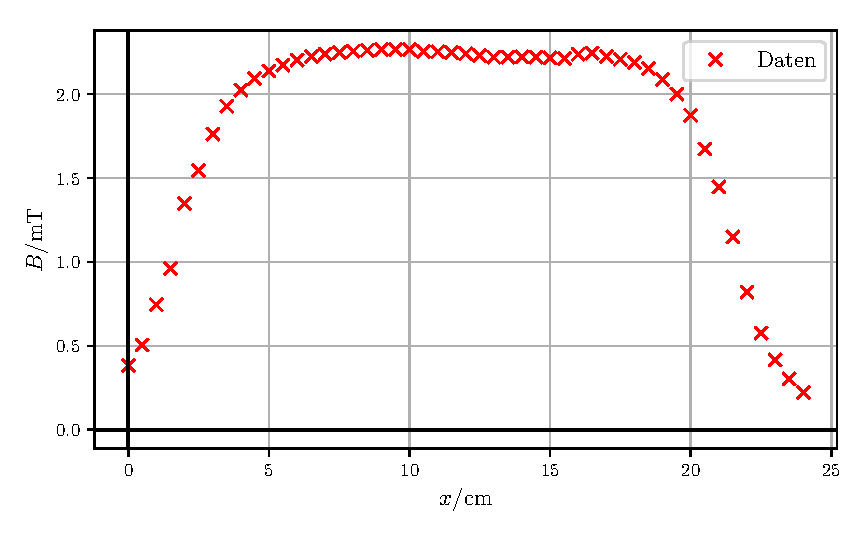
\includegraphics{build/plota1.pdf}
    \caption{Die magnetische Flussdichte $B$ ist gegen die Position $x$ inner- 
    und außerhalb der langen Spule aufgetragen.}
    \label{plota1}
\end{figure}

%Vergleich der Werte mit Theorie
\noindent 

%Tabelle kurze Spule
\noindent Die kurze Spule hat $\num{100}$ Windungen und eine Länge von
$\SI{12}{\centi\meter}$. %richtige Werte einfügen
In Tabelle \ref{taba2} sind die Werte des magnetischen Flusses $B$
an verschiedenen Stellen $x$ aufgelistet.
Die Werte aus Tabelle \ref{taba2} sind in Abbildung \ref{plota2}
gegeneinadner aufgetragen.
\begin{table}\caption{Die Index Werte entsprechen der Höhe, die bei der jeweiligen Ablenkspannung $U_\text{d}$ und der Beschleunigungsspannung $U_\text{B} = \SI{230}{\volt}$ gemessen wurden. Der Indexwert $1$ entspricht einer Höhe von $\SI{0.6}{\centi\meter}$.}
\label{taba2}
\centering
\sisetup{round-mode = places, round-precision=1, round-integer-to-decimal=true}
\begin{tabular}{S[]S[]} 
\toprule
{Index} & {$U_\text{d} / \si{\volt}$}\\
\midrule
1.0 & -25.8\\
2.0 & -21.8\\
3.0 & -17.8\\
4.0 & -13.5\\
5.0 & -9.4\\
6.0 & -5.2\\
7.0 & -1.0\\
8.0 & 3.4\\
9.0 & 7.8\\
\bottomrule
\end{tabular}\end{table}

%Grafik kurze Spule (xB-Diagramm)
\begin{figure}
    \centering
    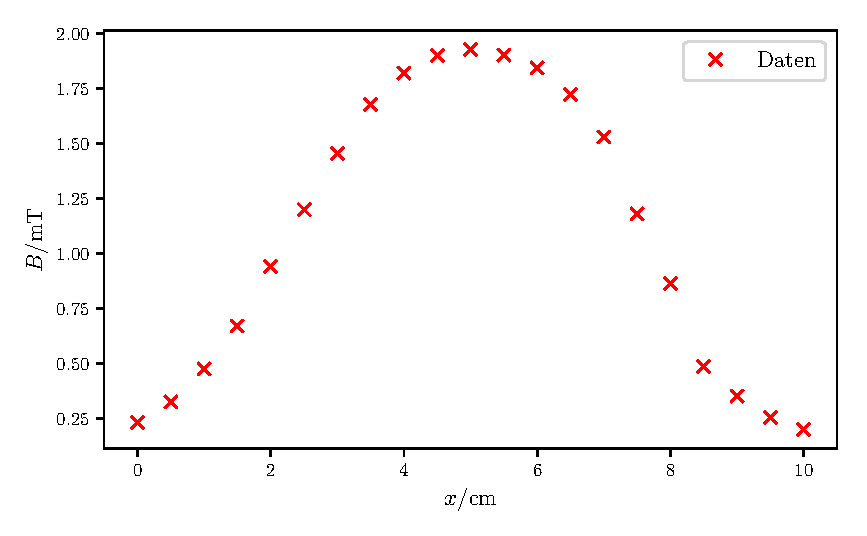
\includegraphics{build/plota2.pdf}
    \caption{Die magnetische Flussdichte $B$ ist gegen die Position $x$ inner-
    und außerhalb der kurzen Spule aufgetragen.}
    \label{plota2}
\end{figure}

%Vergleich der Werte mit Theorie
\noindent 

\subsection{Magnetische Flussdichte eines Spulenpaares}
%ABSTAND=RADIUS
%Tabelle mit I=4A
Zunächst wird der Abstand der beiden Spulen so festgelegt, dass
er den Radien der Spulen entspricht. Es handelt sich um ein
Helmholtz-Spulenpaar.
Es wird eine Stromstärke von $I = \SI{4}{\ampere}$ für die
Messung eingestellt.
Die Werte des magnetischen Flusses an verschiedenen Stellen
$x$ sind in Tabelle \ref{tabb1} aufgelistet. Dabei wird inner-
und außerhalb der Spulen gemessen.
Dieselben Werte sind in Abbildung \ref{plotb1} gegeneinander
aufgetragen.
\begin{table}\caption{Die Brückenspannungen vor und nach dem Einlegen der Probe und die Widerstände vor- und nachher.}
\label{tabb1}
\centering
\sisetup{round-mode = places, round-precision=2, round-integer-to-decimal=true}
\begin{tabular}{S[]S[]S[]S[]} 
\toprule
{U_\text{Br,1} / \si{\milli\volt}} & {U_\text{Br,2} / \si{\milli\volt}} & {5 \cdot R_\text{1} / \si{\milli\ohm}} & {5 \cdot R_\text{2} / \si{\milli\ohm}}\\
\midrule
0.014 & 0.016 & 637.0 & 623.0\\
0.014 & 0.0145 & 623.0 & 619.0\\
0.014 & 0.015 & 630.0 & 616.0\\
\bottomrule
\end{tabular}\end{table}

%Grafik (xB-Diagramm)
\begin{figure}
    \centering
    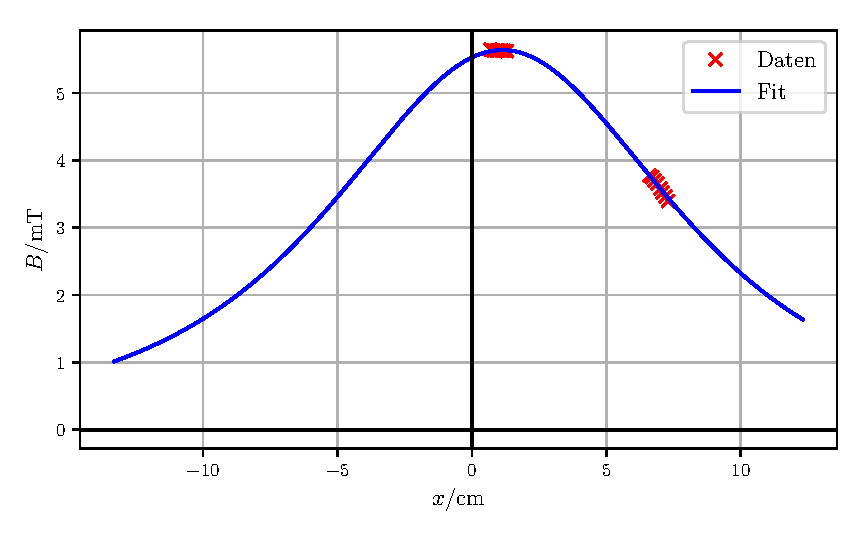
\includegraphics{build/plotb1.pdf}
    \caption{Die magnetische Flussdichte $B$ ist gegen die Position $x$ inner-
    und außerhalb des Helmholtz-Spulenpaares für eine Stromstärke von
    $\SI{4}{\ampere}$ aufgetragen.}
    \label{plotb1}
\end{figure}

%Vergleich mit Theorie
\noindent

%ABSTAND=DURCHMESSER
%Tabelle mit I=4A
\newline
\noindent Der Abstand der Spulen wird im nächsten Messabschnitt auf den
Durchmesser der Spulen erhöht.
Die eingestellte Stromstärke ist, wie im ersten Teil,
$I = \SI{4}{\ampere}$.
Die magnetische Flussdichte an verschiedenen Stellen $x$ ist
in Tabelle \ref{tabb2} dargestellt.
Diese Werte sind in Abbildung \ref{plotb2} gegeneinadner
aufgetragen.
\begin{table}\caption{Der magnetische Fluss $B$ an verschiedenen Stellen $x$ in- und außerhalb des Spulenpaares bei einem Abstand von \SI{12.5}{\centi\meter} und einem Strom $I$ von \SI{4}{\ampere}.}
\label{tabb2}
\centering
\sisetup{round-mode = places, round-precision=3, round-integer-to-decimal=true}
\begin{tabular}{S[]S[]} 
\toprule
{$B$/ \si{\milli\tesla}} & {$x$/ \si{\centi\meter}}\\
\midrule
2.92 & 1.0\\
2.787 & 1.5\\
2.6740000000000004 & 2.0\\
2.5869999999999997 & 2.5\\
2.522 & 3.0\\
2.48 & 3.5000000000000004\\
2.467 & 4.0\\
2.4810000000000003 & 4.5\\
2.525 & 5.0\\
2.59 & 5.5\\
2.669 & 6.0\\
2.784 & 6.5\\
2.943 & 7.000000000000001\\
3.035 & 7.5\\
2.454 & 13.0\\
2.111 & 13.5\\
1.8940000000000001 & 14.000000000000002\\
1.534 & 14.499999999999998\\
1.3860000000000001 & 15.0\\
\bottomrule
\end{tabular}\end{table}

%Grafik (xB-Diagramm)
\begin{figure}
    \centering
    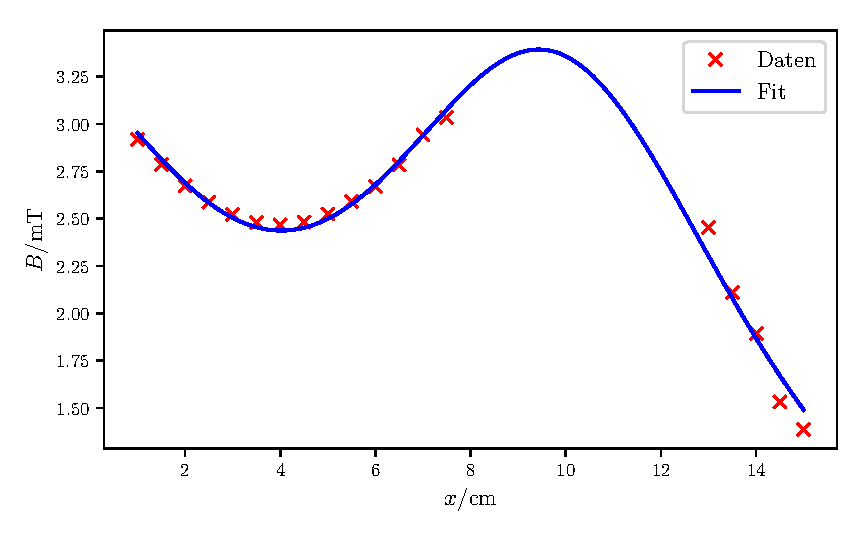
\includegraphics{build/plotb2.pdf}
    \caption{Die magnetische Flussdichte $B$ ist gegen die Position $x$ inner-
    und außerhalb des Spulenpaares mit einem Abstand, der gleich dem Durchmesser
    der Spulen ist, und einer Stromstärke von $\SI{4}{\ampere}$ aufgetragen.}
    \label{plotb2}
\end{figure}

%Vergleich mit Theorie
\noindent

%Tabelle mit I=3A
\noindent Zuletzt wird die angelegte Stromstärke verändert. Der Abstand
der Spulen bleibt unverändert der Durchmesser der Spulen.
Die verwendete Stromstärke ist $I = \SI{3}{\ampere}$.
Der magnetische Fluss an den Positionen $x$ inner- und außerhalb
der Spulen findet sich in Tabelle \ref{tabb3}.
Diese Werte sind in Abbildung \ref{plotb3} gegeneinadner
aufgetragen.
\begin{table}\caption{Der magnetische Fluss $B$ an verschiedenen Stellen $x$ inner- und außerhalb des Spulenpaares bei einem Abstand von \SI{12.5}{\centi\meter} und einem Strom $I$ von \SI{3}{\ampere}.}
\label{tabb3}
\centering
\sisetup{round-mode = places, round-precision=3, round-integer-to-decimal=true}
\begin{tabular}{S[]S[]} 
\toprule
{$B$/ \si{\milli\tesla}} & {$x$/ \si{\centi\meter}}\\
\midrule
2.637 & 1.0\\
2.536 & 1.5\\
2.444 & 2.0\\
2.362 & 2.5\\
2.3040000000000003 & 3.0\\
2.269 & 3.5000000000000004\\
2.2560000000000002 & 4.0\\
2.2680000000000002 & 4.5\\
2.306 & 5.0\\
2.37 & 5.5\\
2.4459999999999997 & 6.0\\
2.552 & 6.5\\
2.657 & 7.000000000000001\\
2.7729999999999997 & 7.5\\
2.42 & 13.0\\
2.265 & 13.5\\
2.065 & 14.000000000000002\\
1.887 & 14.499999999999998\\
1.702 & 15.0\\
1.531 & 15.5\\
\bottomrule
\end{tabular}\end{table}

%Grafik (xB-Diagramm)
\begin{figure}
    \centering
    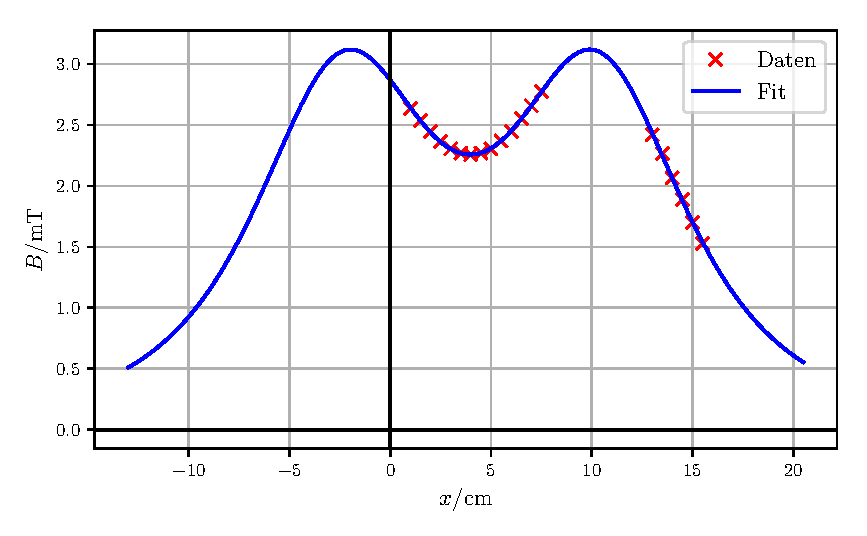
\includegraphics{build/plotb3.pdf}
    \caption{Die magnetische Flussdichte $B$ ist gegen die Position $x$ inner-
    und außerhalb des Spulenpaares mit einem Abstand, der gleich dem Durchmesser
    der Spulen ist, und einer Stromstärke von $\SI{3}{\ampere}$ aufgetragen.}
    \label{plotb3}
\end{figure}

%Vergleich mit Theorie
\noindent

\subsection{Hysteresekurve einer Ringspule mit Luftspalt}
%Tabelle
Der magnetische Fluss $B$ der Ringspule wird im Luftspalt
des Rings gemessen.
In Tabelle \ref{tabc} befinden sich die Werte des magnetischen
Flusses für verschiedene eingestellte Stromstärken.
Diese Werte für den magnetischen Fluss sind in Abbildung
\ref{plotc} gegen die Stromstärke aufgetragen.
\begin{table}\caption{Der Anodenstrom und der Kathodenstrom bei einer Beschleunigungsspannung von $U_\text{B} = \SI{25}{\kilo\volt}$ und einer Kathodenspannung $U_\text{K,1} = \SI{500}{\volt}$ und einer Kathodenspannung $U_\text{K,2} = \SI{300}{\volt}$ bei einem Blendenradius von $r_\text{B} = \SI{5}{\milli\meter}$.}
\label{tabc}
\centering
\sisetup{round-mode = places, round-precision=2, round-integer-to-decimal=true}
\begin{tabular}{S[]S[]S[]} 
\toprule
{$I_\text{K} / \si{\milli\ampere}$} & {$I_\text{K,1} / \si{\nano\ampere}$} & {$I_\text{K,2} / \si{\nano\ampere}$}\\
\midrule
1.0 & 2.6 & 2.4\\
0.95 & 2.5 & 2.4\\
0.9 & 2.4 & 2.2\\
0.85 & 2.3 & 2.1\\
0.8 & 2.2 & 2.0\\
0.75 & 2.1 & 1.9\\
0.7 & 1.9 & 1.8\\
0.65 & 1.8 & 1.6\\
0.6 & 1.6 & 1.5\\
0.55 & 1.5 & 1.4\\
0.5 & 1.4 & 1.3\\
0.45 & 1.2 & 1.2\\
0.4 & 1.1 & 1.0\\
0.35 & 0.9 & 0.9\\
0.3 & 0.8 & 0.8\\
0.25 & 0.6 & 0.6\\
0.2 & 0.5 & 0.5\\
0.15 & 0.4 & 0.4\\
0.1 & 0.1 & 0.2\\
0.05 & 0.1 & 0.1\\
\bottomrule
\end{tabular}\end{table}

%Grafik: Hysteresekurve
\begin{figure}
    \centering
    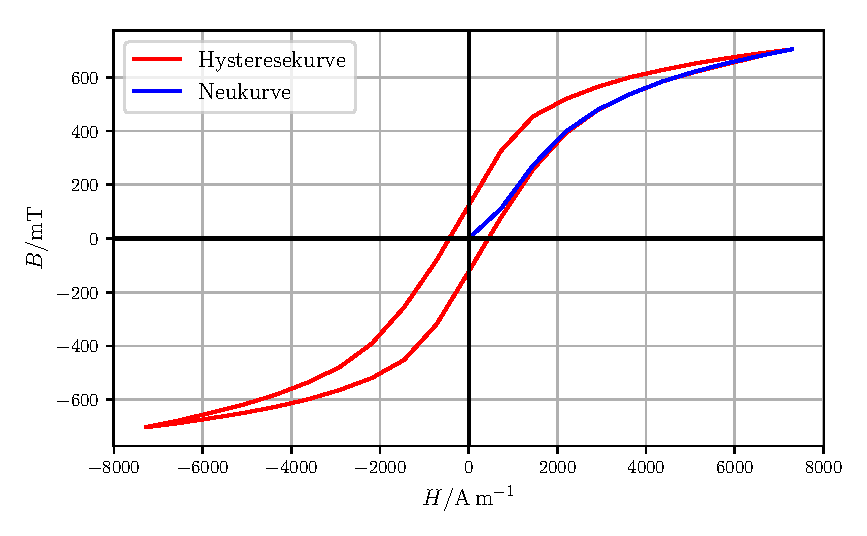
\includegraphics{build/plotc.pdf}
    \caption{Die magnetische Flussdichte $B$ ist gegen die Stromstärke $I$
    aufgetragen. Bei keinem angelegten Strom ist der magnetische Fluss
    gleich Null. Bei Erhöhung der Stromstärke entsteht die Neukurve, bis
    ein Sättigungswert $B_{S}$ (Maximum) erreicht wird. Beim Abschalten des Stroms
    bleibt eine Restmagnetisierung, die Remanenz $B_{r}$ (y-Achsenabschnitt),
    zurück. Ein Gegenfeld $H_{c}$, Koerzitivfeld, hebt diese Magnetisierung wieder
    auf (Schnittpunkt mit der x-Achse). Durch Erhöhung der Stromstärke entsteht
    eine Hysteresekurve.}
    \label{plotc}
\end{figure}

%Werte ablesen:
\noindent Aus der grafischen Darstellung lassen sich verschiedene Faktoren
wie die Sättigungsmagnetisierung $B_{S}$, die Remanenz $B_{r}$ und die
Koerzitivkraft $H_{c}$ ablesen.
Die Sättigungsmagnetisierung ist das Maximum der gemessenen Werte für
die magnetische Flussdichte: $B_{S} = \SI{}{\milli\tesla}$. %Wert
Die negative Sättigungsmagnetisierung ist das Minimum:
$-B_{S} = \SI{}{\milli\tesla}$. %Wert
Die Remanenz ist der obere Schnittpunkt mit der $y$-Achse.
Bestimmt man diesen aus der Grafik, ist die Remanenz also
$B_{r} = \SI{}{\milli\tesla}$. %Wert
Die Koerzitivktaft ist der linke, d.h. kleinere Schnittpunkt mit der Achse.
Hier ist die Koerzitivkraft $H_{c} = \SI{}{\milli\tesla}$. %Wert